\documentclass[12pt]{article}
\usepackage{fullpage,amsmath,amssymb,amsfonts,amsthm}
\usepackage[utf8]{inputenc}
\usepackage[english]{babel}
\usepackage{graphics}
\usepackage{tikz}
\usepackage{pgfplots}

\pgfplotsset{compat=1.8}
\title{Performance Report}

\begin{document}

\maketitle

\begin{figure}[h!]
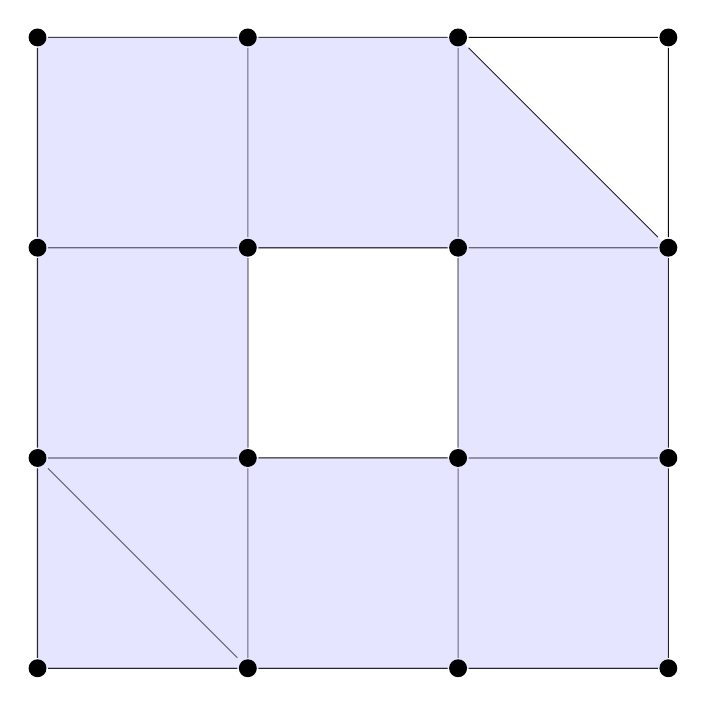
\begin{tikzpicture}[scale=2.67, every node/.style={scale=1.07}]

%vertex labels
\draw
	(0.000000,0.000000) node (v0) {}
	(1.000000,0.000000) node (v1) {}
	(0.000000,1.000000) node (v2) {}
	(1.000000,1.000000) node (v3) {}
	(2.000000,0.000000) node (v4) {}
	(2.000000,1.000000) node (v5) {}
	(3.000000,0.000000) node (v6) {}
	(3.000000,1.000000) node (v7) {}
	(0.000000,2.000000) node (v8) {}
	(1.000000,2.000000) node (v9) {}
	(2.000000,2.000000) node (v10) {}
	(3.000000,2.000000) node (v11) {}
	(0.000000,3.000000) node (v12) {}
	(1.000000,3.000000) node (v13) {}
	(2.000000,3.000000) node (v14) {}
	(3.000000,3.000000) node (v15) {};

%plot non-open edges
\draw
	(v0)--(v1)
	(v1)--(v3)
	(v3)--(v2)
	(v2)--(v0)
	(v1)--(v4)
	(v4)--(v5)
	(v5)--(v3)
	(v4)--(v6)
	(v6)--(v7)
	(v7)--(v5)
	(v3)--(v9)
	(v9)--(v8)
	(v8)--(v2)
	(v5)--(v10)
	(v10)--(v9)
	(v7)--(v11)
	(v11)--(v10)
	(v9)--(v13)
	(v13)--(v12)
	(v12)--(v8)
	(v10)--(v14)
	(v14)--(v13)
	(v11)--(v15)
	(v15)--(v14)
	(v1)--(v2)
	(v11)--(v14);

%plot open edges
\draw[very thick, dashed];

%fill faces
\fill[color=blue!20, opacity=.5] 
	(v0.center)--(v1.center)--(v3.center)--(v2.center)--cycle
	(v1.center)--(v4.center)--(v5.center)--(v3.center)--cycle
	(v4.center)--(v6.center)--(v7.center)--(v5.center)--cycle
	(v3.center)--(v2.center)--(v8.center)--(v9.center)--cycle
	(v7.center)--(v5.center)--(v10.center)--(v11.center)--cycle
	(v9.center)--(v8.center)--(v12.center)--(v13.center)--cycle
	(v10.center)--(v9.center)--(v13.center)--(v14.center)--cycle
	(v11.center)--(v10.center)--(v14.center)--(v15.center)--cycle
	(v2.center)--(v0.center)--(v1.center)--cycle
	(v15.center)--(v14.center)--(v11.center)--cycle;

%plot non-open vertices
\draw
	(v0) node[draw, circle, inner sep=2pt, fill=black] {}
	(v1) node[draw, circle, inner sep=2pt, fill=black] {}
	(v2) node[draw, circle, inner sep=2pt, fill=black] {}
	(v3) node[draw, circle, inner sep=2pt, fill=black] {}
	(v4) node[draw, circle, inner sep=2pt, fill=black] {}
	(v5) node[draw, circle, inner sep=2pt, fill=black] {}
	(v6) node[draw, circle, inner sep=2pt, fill=black] {}
	(v7) node[draw, circle, inner sep=2pt, fill=black] {}
	(v8) node[draw, circle, inner sep=2pt, fill=black] {}
	(v9) node[draw, circle, inner sep=2pt, fill=black] {}
	(v10) node[draw, circle, inner sep=2pt, fill=black] {}
	(v11) node[draw, circle, inner sep=2pt, fill=black] {}
	(v12) node[draw, circle, inner sep=2pt, fill=black] {}
	(v13) node[draw, circle, inner sep=2pt, fill=black] {}
	(v14) node[draw, circle, inner sep=2pt, fill=black] {}
	(v15) node[draw, circle, inner sep=2pt, fill=black] {};

%plot open vertices
\draw;

\end{tikzpicture}
\hspace{.2cm}
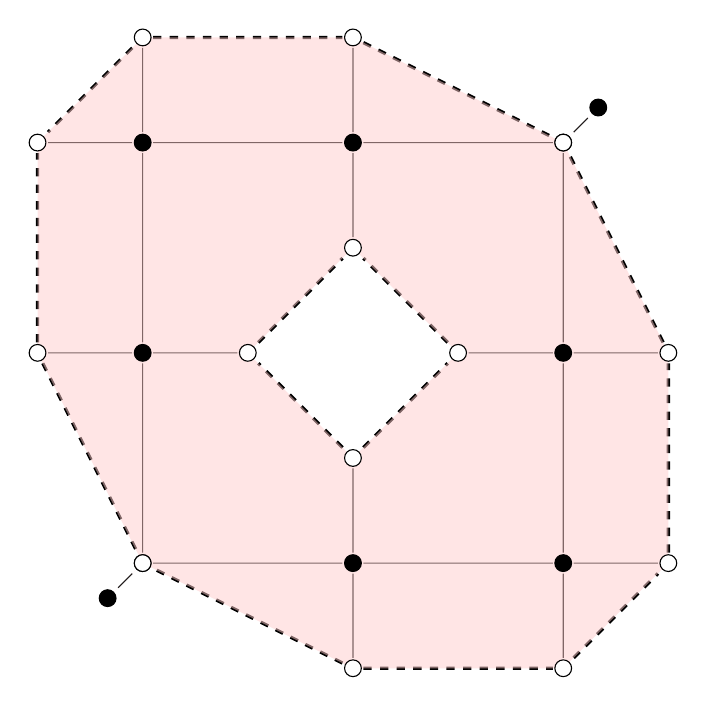
\begin{tikzpicture}[scale=2.67, every node/.style={scale=1.07}]

%vertex labels
\draw
	(0.500000,0.500000) node (v0) {}
	(1.500000,0.500000) node (v1) {}
	(2.500000,0.500000) node (v2) {}
	(0.500000,1.500000) node (v3) {}
	(2.500000,1.500000) node (v4) {}
	(0.500000,2.500000) node (v5) {}
	(1.500000,2.500000) node (v6) {}
	(2.500000,2.500000) node (v7) {}
	(0.333333,0.333333) node (v8) {}
	(2.666667,2.666667) node (v9) {}
	(1.500000,0.000000) node (v10) {}
	(1.500000,1.000000) node (v11) {}
	(2.500000,0.000000) node (v12) {}
	(3.000000,0.500000) node (v13) {}
	(1.000000,1.500000) node (v14) {}
	(0.000000,1.500000) node (v15) {}
	(2.000000,1.500000) node (v16) {}
	(1.500000,2.000000) node (v17) {}
	(3.000000,1.500000) node (v18) {}
	(0.500000,3.000000) node (v19) {}
	(0.000000,2.500000) node (v20) {}
	(1.500000,3.000000) node (v21) {}
	(0.500000,0.500000) node (v22) {}
	(2.500000,2.500000) node (v23) {};

%plot non-open edges
\draw
	(v0)--(v8)
	(v0)--(v1)
	(v0)--(v3)
	(v0)--(v8)
	(v1)--(v10)
	(v1)--(v2)
	(v1)--(v11)
	(v2)--(v12)
	(v2)--(v13)
	(v2)--(v4)
	(v3)--(v14)
	(v3)--(v5)
	(v3)--(v15)
	(v4)--(v16)
	(v6)--(v17)
	(v4)--(v18)
	(v4)--(v7)
	(v5)--(v6)
	(v5)--(v19)
	(v5)--(v20)
	(v6)--(v7)
	(v6)--(v21)
	(v7)--(v9)
	(v7)--(v9)
	(v8)--(v22)
	(v9)--(v23);

%plot open edges
\draw[very thick, dashed]
	(v10)--(v22)
	(v15)--(v22)
	(v11)--(v14)
	(v10)--(v12)
	(v11)--(v16)
	(v12)--(v13)
	(v13)--(v18)
	(v15)--(v20)
	(v14)--(v17)
	(v16)--(v17)
	(v18)--(v23)
	(v19)--(v20)
	(v19)--(v21)
	(v21)--(v23);

%fill faces
\fill[color=red!20, opacity=.5] 
	(v0.center)--(v8.center)--cycle
	(v0.center)--(v8.center)--(v22.center)--(v10.center)--(v1.center)--cycle
	(v0.center)--(v3.center)--(v15.center)--(v22.center)--(v8.center)--cycle
	(v0.center)--(v1.center)--(v11.center)--(v14.center)--(v3.center)--cycle
	(v1.center)--(v10.center)--(v12.center)--(v2.center)--cycle
	(v1.center)--(v2.center)--(v4.center)--(v16.center)--(v11.center)--cycle
	(v2.center)--(v12.center)--(v13.center)--cycle
	(v2.center)--(v13.center)--(v18.center)--(v4.center)--cycle
	(v3.center)--(v5.center)--(v20.center)--(v15.center)--cycle
	(v3.center)--(v14.center)--(v17.center)--(v6.center)--(v5.center)--cycle
	(v4.center)--(v16.center)--(v17.center)--(v6.center)--(v7.center)--cycle
	(v4.center)--(v18.center)--(v23.center)--(v9.center)--(v7.center)--cycle
	(v5.center)--(v19.center)--(v20.center)--cycle
	(v5.center)--(v6.center)--(v21.center)--(v19.center)--cycle
	(v6.center)--(v7.center)--(v9.center)--(v23.center)--(v21.center)--cycle
	(v7.center)--(v9.center)--cycle;

%plot non-open vertices
\draw
	(v0) node[draw, circle, inner sep=2pt, fill=black] {}
	(v1) node[draw, circle, inner sep=2pt, fill=black] {}
	(v2) node[draw, circle, inner sep=2pt, fill=black] {}
	(v3) node[draw, circle, inner sep=2pt, fill=black] {}
	(v4) node[draw, circle, inner sep=2pt, fill=black] {}
	(v5) node[draw, circle, inner sep=2pt, fill=black] {}
	(v6) node[draw, circle, inner sep=2pt, fill=black] {}
	(v7) node[draw, circle, inner sep=2pt, fill=black] {}
	(v8) node[draw, circle, inner sep=2pt, fill=black] {}
	(v9) node[draw, circle, inner sep=2pt, fill=black] {};

%plot open vertices
\draw
	(v10) node[draw, circle, inner sep=2pt, fill=white] {}
	(v11) node[draw, circle, inner sep=2pt, fill=white] {}
	(v12) node[draw, circle, inner sep=2pt, fill=white] {}
	(v13) node[draw, circle, inner sep=2pt, fill=white] {}
	(v14) node[draw, circle, inner sep=2pt, fill=white] {}
	(v15) node[draw, circle, inner sep=2pt, fill=white] {}
	(v16) node[draw, circle, inner sep=2pt, fill=white] {}
	(v17) node[draw, circle, inner sep=2pt, fill=white] {}
	(v18) node[draw, circle, inner sep=2pt, fill=white] {}
	(v19) node[draw, circle, inner sep=2pt, fill=white] {}
	(v20) node[draw, circle, inner sep=2pt, fill=white] {}
	(v21) node[draw, circle, inner sep=2pt, fill=white] {}
	(v22) node[draw, circle, inner sep=2pt, fill=white] {}
	(v23) node[draw, circle, inner sep=2pt, fill=white] {};

\end{tikzpicture}
\caption{The tiling and its dual tiling}
\end{figure}
\vspace{.2cm}

\newpage
\begin{table}[h]
\centering
\begin{tabular}{c c}
\hline
Number of physical qubits & $n = 26$ \\
\hline
Number of logical qubits & $k = 1$\\
\hline
Overhead & $n/k = 26.00$\\
\hline
\end{tabular}
\caption{Error-correction overhead}
\end{table}
\vspace{.3cm}


\begin{table}[h]
\centering
\begin{tabular}{c c}
\hline
weight & number of $Z$-measurements\\
\hline
3 & 2\\
4 & 8\\
\hline
\hline
weight & number of $X$-measurements\\
\hline
2 & 4\\
3 & 4\\
4 & 8\\
\hline
\end{tabular}
\caption{Measurements weight distribution}
\end{table}
\vspace{.3cm}


\newpage
\begin{figure}[h!]
\centering

\begin{tikzpicture}[scale=1.00, every node/.style={scale=1.00}]

\begin{semilogyaxis}
[
    grid= major,
    xlabel = {erasure probability},
    ylabel = {logical error rate after decoding},
    xmin = 0.00, xmax = 0.30,
    ymax = 1,
    legend entries={D},
    legend pos={south east},
]

\addplot+[
    error bars/.cd,
    y dir=both,
    y explicit,
    ]table[x index=0, y index=1, y error index=4]{../results/perf_D_9_8_2020_15_49_23.txt};

\end{semilogyaxis}


\end{tikzpicture}
\caption{Logical error rate after decoding}
\end{figure}
\vspace{.2cm}

\begin{figure}[h!]
\begin{tikzpicture}[scale=1.00, every node/.style={scale=1.00}]

\begin{semilogyaxis}
[
    grid= major,
    xlabel = {erasure probability},
    ylabel = {logical error rate after decoding},
    xmin = 0.00, xmax = 0.30,
    ymax = 1,
    legend entries={D},
    legend pos={south east},
]

\addplot+[
    error bars/.cd,
    y dir=both,
    y explicit,
    ]table[x index=0, y index=5, y error index=8]{../results/perf_D_9_8_2020_15_49_23.txt};

\end{semilogyaxis}


\end{tikzpicture}
\begin{tikzpicture}[scale=1.00, every node/.style={scale=1.00}]

\begin{semilogyaxis}
[
    grid= major,
    xlabel = {erasure probability},
    ylabel = {logical error rate after decoding},
    xmin = 0.00, xmax = 0.30,
    ymax = 1,
    legend entries={D},
    legend pos={south east},
]

\addplot+[
    error bars/.cd,
    y dir=both,
    y explicit,
    ]table[x index=0, y index=9, y error index=12]{../results/perf_D_9_8_2020_15_49_23.txt};

\end{semilogyaxis}


\end{tikzpicture}
\caption{Left: Z-logical error rate after decoding. Right: X-logical error rate after decoding}
\end{figure}
\vspace{.2cm}


\vspace{2cm}
Total simulation time: $< 1$ second.
\end{document}